\univlogo

{\Huge April 7}\vspace{5mm}

\section*{After-class assignments}

\subsection*{4.4}

Implement the delta training rule for a two-input linear unit. Train it to fit the target concept $-2 + x_1+ 2x_2 > 0$. Plot the error E as a function of the number of training iterations. Plot the decision surface after 5, 10, 50, 100, \dots , iterations.

(a) Try this using various constant values for $\eta$ and using a decaying learning rate of $\eta_0/i$ for the $i$th iteration. Which works better?

(b) Try incremental and batch learning. Which converges more quickly? Consider both number of weight updates and total execution time.

So I ran the following code:

\begin{python}
import numpy as np
import pandas as pd
import neurolab as nl
import matplotlib.pyplot as plt
# Generate 1000 data randomly
X = np.random.uniform(low=-10, high=10, size=(1000, 2))

# Generate Labels -2+x1+2x2>0
Y = np.where(-2 + X[:, 0] + 2 * X[:, 1] > 0, 1, -1)

# Save to file
np.savetxt("data.csv", np.column_stack([X, Y]), delimiter=",")

# Read file
data = pd.read_csv("data.csv", header=None)

# Read data and labels
x = data.iloc[:, :-1].values
y = data.iloc[:, -1].values.reshape(-1, 1)

# Plot input data
plt.figure()
plt.scatter(x[:,0], x[:,1])
plt.xlabel('X-axis')
plt.ylabel('Y-axis')
plt.title('Input data')

# Define a perceptron with 2 inputs;
# Each element of the list in the first argument 
# specifies the min and max values of the inputs
#  Tanh (Use 1 and -1 as labels)
perceptron = nl.net.newp([[-10, 10],[-10, 10]], 1, transf=nl.trans.TanSig())

# Train the perceptron
error = perceptron.train(x, y, epochs=5000, show=True, lr=0.1)

# plot results
plt.figure()
plt.plot(error)
plt.xlabel('Number of epochs')
plt.ylabel('Training error')
plt.grid()
plt.title('Training error progress')
plt.show()

\end{python}

At first I set $\eta=0.1$ and it costs over 2000 epochs to reach that $error < 0.01$.

\begin{figure}[H]
    \centering
    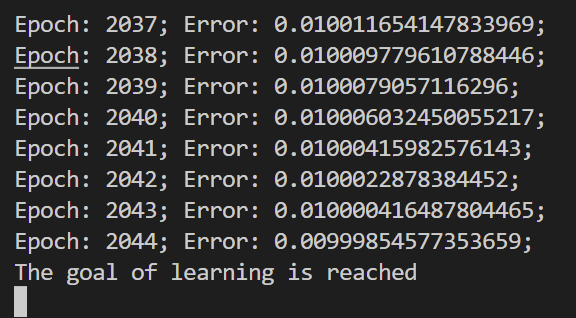
\includegraphics[width=0.6\textwidth]{./2023April/eta0.1.png}
    \caption{$\eta$=0.1, 2000+ epochs}
    \label{eta0.1}
\end{figure}

It is surprising that it take such long time to train a perceptron under a linear model. So I change $\eta=1$

\begin{figure}[H]
    \centering
    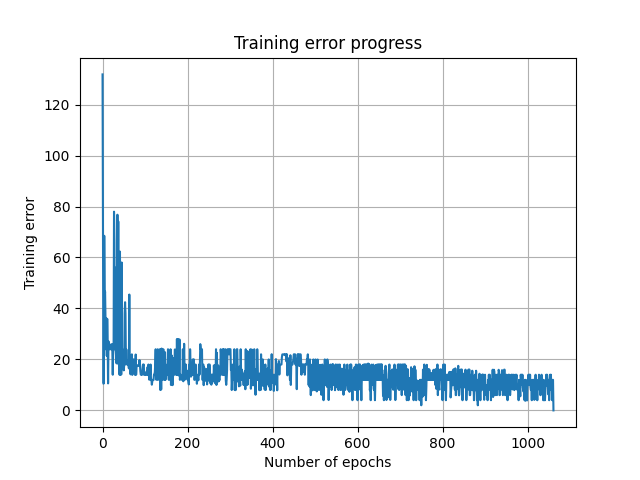
\includegraphics[width=0.6\textwidth]{./2023April/graphEta1.png}
    \caption{$\eta$=1, over 1k epochs}
    \label{eta1}
\end{figure}

We can see that the number of iterations becomes less and there is an oscillation in the gradient descent.

Input data and training results are shown below:

\begin{figure}[H]
    \centering
    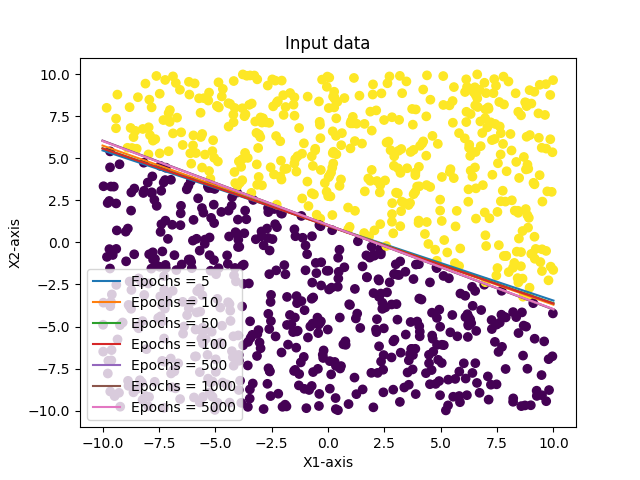
\includegraphics[width=0.6\textwidth]{./2023April/input data.png}
    \caption{Input data and training results}
    \label{input data}
\end{figure}

The training error progress is shown below:

\begin{figure}[H]
    \centering
    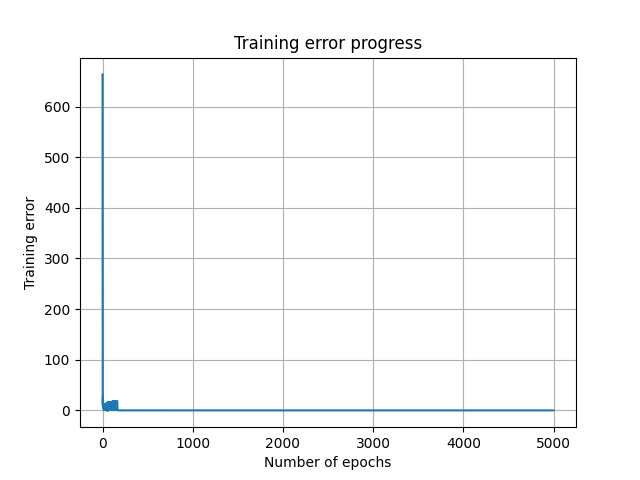
\includegraphics[width=0.6\textwidth]{./2023April/training error progress.png}
    \caption{Training error progress}
    \label{training error progress}
\end{figure}

Technically speaking, batch learning converges more quickly, if appropriate learning rate selected. Incremental learning is less likely to oscilate but requires more number of weight updates.